\documentclass[a4paper,12pt, oneside]{book}

%\usepackage{fullpage}
\usepackage[T1]{fontenc}
\usepackage[italian]{babel}
\usepackage[utf8]{inputenc}
\usepackage{amssymb}
\usepackage{amsthm}
\usepackage{graphics}
\usepackage{amsfonts}
\usepackage{listings}
\usepackage{amsmath}
\usepackage{amstext}
\usepackage{engrec}
\usepackage{rotating}
\usepackage[safe,extra]{tipa}
\usepackage{showkeys}
\usepackage{multirow}
\usepackage{hyperref}
\usepackage{microtype}
\usepackage{enumerate}
\usepackage{braket}
\usepackage{marginnote}
\usepackage{pgfplots}
\usepackage{cancel}
\usepackage{polynom}
\usepackage{booktabs}
\usepackage{enumitem}
\usepackage{framed}
\usepackage{pdfpages}
\usepackage{pgfplots}
\usepackage[cache=false]{minted}
 \usepackage[usenames,dvipsnames, pdf]{pstricks}
 \usepackage{epsfig}
 \usepackage{pst-grad} % For gradients
 \usepackage{pst-plot} % For axes
 \usepackage[space]{grffile} % For spaces in paths
 \usepackage{etoolbox} % For spaces in paths
 \makeatletter % For spaces in paths
 \patchcmd\Gread@eps{\@inputcheck#1 }{\@inputcheck"#1"\relax}{}{}
 \makeatother
\usepackage{fancyhdr}
\pagestyle{fancy}
\fancyhead[LE,RO]{\slshape \rightmark}
\fancyhead[LO,RE]{\slshape \leftmark}
\fancyfoot[C]{\thepage}



\title{Analisi e Progettazione del Software}
\author{UniShare\\\\Davide Cozzi\\\href{https://t.me/dlcgold}{@dlcgold}\\\\Gabriele De Rosa\\\href{https://t.me/derogab}{@derogab} \\\\Federica Di Lauro\\\href{https://t.me/f_dila}{@f\textunderscore dila}}
\date{}

\pgfplotsset{compat=1.13}
\begin{document}
\maketitle

\definecolor{shadecolor}{gray}{0.80}

\newtheorem{teorema}{Teorema}
\newtheorem{definizione}{Definizione}
\newtheorem{esempio}{Esempio}
\newtheorem{corollario}{Corollario}
\newtheorem{lemma}{Lemma}
\newtheorem{osservazione}{Osservazione}
\newtheorem{nota}{Nota}
\newtheorem{esercizio}{Esercizio}
\tableofcontents
\renewcommand{\chaptermark}[1]{%
\markboth{\chaptername
\ \thechapter.\ #1}{}}
\renewcommand{\sectionmark}[1]{\markright{\thesection.\ #1}}
\chapter{Introduzione}
\textbf{Questi appunti sono presi durante le lezioni in aula. Per quanto sia stata fatta una revisione è altamente probabile (praticamente certo) che possano contenere errori, sia di stampa che di vero e proprio contenuto. Per eventuali proposte di correzione effettuare una pull request. Link: } \url{https://github.com/dlcgold/Appunti}.\\
\textbf{Grazie mille e buono studio!}
\chapter{Introduzione all'Ingegneria del software}
Durante il corso di Analisi e Progettazione del software si analizzano i modelli e i principi per lo sviluppo di un 
software mantenibile, andando anche ad analizzare, in maniera sommaria, anche tutti gli strumenti di 
ingegneria del software, necessari per lo sviluppo ottimale di un software.

In questo corso studieremo in dettaglio i seguenti argomenti:
\begin{itemize}
    \item introduzione all'ingegneria del software
    \item progettazione sistemi orientati ad oggetti
    \item modellazione a dominio
    \item UML e analisi dei casi d'uso
    \item design pattern
    \item sviluppo test-driven(cenni)
    \item code smell e refactoring(cenni)
\end{itemize}
Il software, è l'insieme delle componenti modificabili e non fisiche di un calcolatore, viene diviso in due categorie:
\begin{description}
    \item [generici], per un ampio range di clienti, come ad esempio gli elaboratori di testi
    \item [custom], per un singolo cliente, come ad esempio i gestionali specifici di un impresa
\end{description}
Questa differenza si sta sempre più assottiliando in quanto recentemente varie aziende stanno sviluppando un 
software generico, che viene poi adattato in base alle esigenze del singolo cliente, 
come ad esempio i software Oracle e Sas.

Nello sviluppo di software si utlizza spesso una base pre-esistente, infatti l'ingegneria del software si occupa
di tutti gli aspetti per lo sviluppo del software, sfruttando di solito una base preesistente. \newline
Di solito quando si sviluppa un software si presuppone che abbia una durata di alcuni anni, con la predispozione
al cambiamento e all'introduzione di nuove features infatti un software per essere utile deve essere continuamente cambiato.

Si hanno due tipologie di progetti:
\begin{enumerate}
        \item \textbf{progetti di routine}, con soluzione di problemi e riuso di vecchio codice
        \item \textbf{progetti innovativi}, con soluzioni nuovi
\end{enumerate}
e solitamente l'ingegneria del software si occupa principalmente di progetti innovativi 
con specifiche del progetto variabili, con la presenza di cambiamenti continui e ovviamente 
non è uguale nè similare con l'ingegneria tradizionale.

Un programmatore normalmente lavora da solo, su un programma completo con specifiche note mentre un ingegnere del software
lavora in gruppo, progetta componenti e l'architettura e identifica requisiti e specifiche.
Il costo del software spesso supera quello hardware %aggiungere grafico

Nello sviluppo di un software si hanno le seguenti fasi di sviluppo:
\begin{itemize}
    \item \textbf{analisi dei requisiti}, che indica cosa deve fare il sistema
    \item \textbf{progettazione}, progetto del sistema d implementare 
    \item \textbf{sviluppo}, produzione del sistema software
    \item \textbf{convalida}, verifica dei requisiti del cliente
    \item \textbf{evoluzione}, evoluzione al cambiare di requisiti del cliente
\end{itemize} 
Esistono dei sistemi software per l'automazione delle attività svolte nel progetto software, 
i cosiddetti \textbf{CASE} (Computer-Aided Software Engineering) che si dividono in:
\begin{description}
    \item [CASE di alto livello] per il supporto alle prime attività di processo come la raccolta requisiti e la progettazione
    \item [CASE di basso livello] per il supporto alle ultime attività di processo come la programmazione,
                                  il debugging, testing e reverse engineering
\end{description}
Nella figure X1 e X2  si hanno delle risposte alle comuni domande sull'ingegneria del software e le caratteristiche
di un ottimo software, necessario per mantenerlo facilmente modificabile nel tempo.

Nello sviluppo di un software, qualsiasi tipologia esso sia, prevede i seguenti aspetti in comune:
\begin{description}
    \item [specifiche del software] vengono definite le specifiche e analizzato in dettaglio il comportamento 
            e le funzionalità richieste da sviluppare
    \item [sviluppo del software] viene effettivamente implementato e progettato il codice, attraverso i tools di sviluppo,
            rispettando le specifiche previste nella fase precedente.
    \item [convalida del software] viene testato il software sviluppato nella fase precedente, al f
    \item [evoluzione del software] viene mantenuto ed evoluto il software, al fine di riflettere i cambiamenti e delle
            funzionalità richieste dal cliente;è la fase più critica e costosa, dato che a volte la manutenzione richiede
            di sistemare e correggere gli errori e/o il cattivo design del progetto.
\end{description}
Il software deve essere accettato dagli utenti per i quali è stato sviluppato per cui deve essere comprensibile, 
usabile e compatibile con altri sistemi, oltre a dover essere mantenibile, affidabile ma soprattutto efficente.

Esiste un codice etico, \textbf{ACM/IEEE}, con otto principi legati al comportamento degli ingegneri del software
ed è fondamentale seguirlo dato che fornisce informazioni su come risolvere i problemi etici collegati
a tutti i progetti software, come le informazioni da fornire all'esterno ed altri aspetti.

Un \textbf{sistema} è una collezione significativa di componenti interrelati che lavorano assieme per realizzare
un obiettivo comune, quindi include software e parti meccaniche o elettriche;inoltre si ha che i vari 
componenti possono dipendere da altri componenti e che le proprietà e il comportamento dei vari componenti
sono intrinsecamente correlati, quindi si hanno due macro categorie:
\begin{enumerate}
    \item \textbf{sistemi tecnico-informatici}, in cui sono inclusi hardware e software ma non gli operatori e i
        processi operazionali, dove sono presenti le \textbf{proprietà emergenti}, dipendenti dalle sue componenti
        e le relazioni tra esse, misurabili soltanto sul sistema finale.\newline
        Inoltre i sistemi tecnici sono non-deterministici, in quanto dato lo stesso input non è detto che restituisca
        lo stesso output, in quanto il risultato è spesso dipendente dal comportamento degli operatori umani.
    \item \textbf{sistemi socio-tecnici}, comprendente uno o più sistemi tecnici, assieme ai processi operazionali 
        e agli operatori, sono fortemente condizionati da politiche aziendali e regole.\newline        
        I sistemi Socio-tecnici sono sistemi pensati per raggiungere obiettivi aziendali o organizzativi 
        e bisogna comprendere a fondo l'ambiente organizzatico nel quale un certo sistema è usato.
\end{enumerate}
Vediamo qualche proprietà emergente:
\begin{itemize}
    \item \textbf{volume:} il volume di un sistema varia a seconda di come sono disposti
        e collegati i componenti che lo formano.
    \item \textbf{affidabilità:} l'affidabilità del sistema dipende dall'affidabilità dei suoi componenti,
        ma interazioni impreviste possono produrre nuovi fallimenti 
        e quindi influenzare l'affidabilità dell'intero sistema
    \item \textbf{protezione:} la protezione del sistema è una proprietà complessa 
        che non può essere facilmente misurata, in quanto in futuro potrebbero essere inventati
        nuove modalità di accesso e/o attacco che rendeno meno protetto il software.
    \item \textbf{riparabilità:} questa proprietà riflette la facilità con cui è possibile
        correggere un problema e ciò dipende dalla possibilità di diagnosticare il problema
        e soprattutto di accedere, modificare o sostituire i componenti difettosi.
    \item \textbf{usabilità:} questa proprietà mostra la facilità d‘uso del sistema e dipende dai componenti del
            sistema tecnico, dai suoi operatori e dal suo ambiente operativo.
\end{itemize}
Oltre a questi sistemi software standard, sono presenti i \textbf{sistemi critici}, 
in cui fondamentalmente non sono ammessi errori e malfunzionamenti altrimenti causano dei gravi problemi
se non morti, per questo le specifiche avvengono in linguaggio il più possibile formale possibile
e usano un modello di sviluppo a cascata, inefficente per gli altri sistemi software.

Abbiamo tre esempi di sistemi critici:
\begin{enumerate}
    \item \textbf{sistemi safety-critical} dove i fallimenti comportano rischi ambientali
        o perdite di vite umane, come ad esempio un sistema di controllo per un impianto chimico.
    \item \textbf{sistemi mission-critical} dove i fallimenti possono causare il fallimento 
        di attività a obiettivi diretti, come un sistema di navigazione di un veicolo spaziale.
    \item \textbf{sistemi business-critical} dove i fallimenti possono risultare 
        in perdite di denaro sostenute, come ad esempio un sistema bancario.
\end{enumerate}
I fallimenti di un software, sia che fossero piccoli che grandi, possono essere di diversi tipi:
\begin{itemize}
\item \textbf{fallimenti hardware}, errori di progetto, produzione o "consumo"
\item \textbf{fallimenti software}, errori di specifica, progetto, implementazione
\item \textbf{errori operativi}, errori commessi da operatori umani (forse una delle maggiori cause di fallimenti)
\end{itemize}
Nei sistemi critici, generalmente la fidatezza è la più importante proprietà del sistema 
in quanto si ha un alto costo dei fallimenti ed esso riflette il livello di confidenza
che l'utente ha verso il sistema, cosa leggermente diversa dall'utilità,
ossia la sicurezza di non avere problemi e/o intrusioni da parte di persone esterne.

Il costo dei fallimenti nei sistemi critici è così alto che i metodi di ingegneria del software
non sono cost-effective per cui si utilizza un modello a cascata, in quanto si devono fare prima 
tutte le analisi, prima di poter implementare e testare il sistema e soprattutto si spende un
sacco di soldi per il testing e le analisi per convalidare la fidatezza necessaria da raggiungere.

\section{Modelli di Processo}
Il modello di un processo software è una rappresentazione semplificata del processo, basata su un aspetto specifico:
\begin{itemize}
    \item \textbf{modello a flusso di lavoro (Workflow)} per una sequenza di attività
    \item \textbf{modello a flusso di dati (Data-flow)} per il flusso delle informazioni
    \item \textbf{modello ruolo/azione (role/action)} per decidere i vari ruoli
\end{itemize}
si hanno poi tre modelli generici:
\begin{enumerate}
    \item \textbf{modello a cascata (waterfall)}: modello in cui le diverse fasi, come si nota nella figura XDDDD,
        avvengono  in sequenza, dove i problemi e/o mancanze di interpretazioni si notano verso 
        la fine dello sviluppo, nella fase di test e/o consegna, e ciò comporta una modifica di una 
        o più fasi precedenti dello sviluppo, con notevoli aggravi di costi e tempestiche.\newline
        È stato il primo modello di sviluppo, ma a partire dagli anni 90 si comprese che la 
        maggioranza dei fallimenti dei software era da imputare al fatto di cercare di definire tutti
        i requisiti prima di sviluppare, cosa che è difficile da fare in maniera efficace in sistemi 
        variabili nel tempo, come quasi tutti i sistemi software da sviluppare e/o già sviluppati.
    \item \textbf{modello iterativo (Iterative development)}: modello in cui le fasi di sviluppo avvengono
        nel corso del tempo, senza effettuare prima tutta la progettazione e poi l'implementazione, 
        sviluppando versioni sempre più definite del software, portando subito in risalta i problemi 
        e/o le mancate interpretazioni del sistema da sviluppare.\newline
        Prevede diverse implementazioni di questo modello, come ad esempio l'UP, lo Scrum e la modellazione
        agile, in cui il concetto di fondo è quello di conoscere, sviluppare e progettare il sistema a passi
        successivi, al fine di avere ad ogni passo un sottoinsieme del sistema già funzionante e questo
        permette di poter reagire ai cambiamenti dei requisiti e permettere una manutenzione
        mantenibile nel tempo.
    \item \textbf{ingegneria del Software basata sui componenti (CBSE)}
\end{enumerate}
I metodi di ingegneria del software sono l'implementazione dei seguenti modelli generici, e nella
maggioranza si utilizza un modello iterativo, al fine di rendere incrementale lo sviluppo e ridurre
il rischio di fallimento del progetto.
\begin{center}
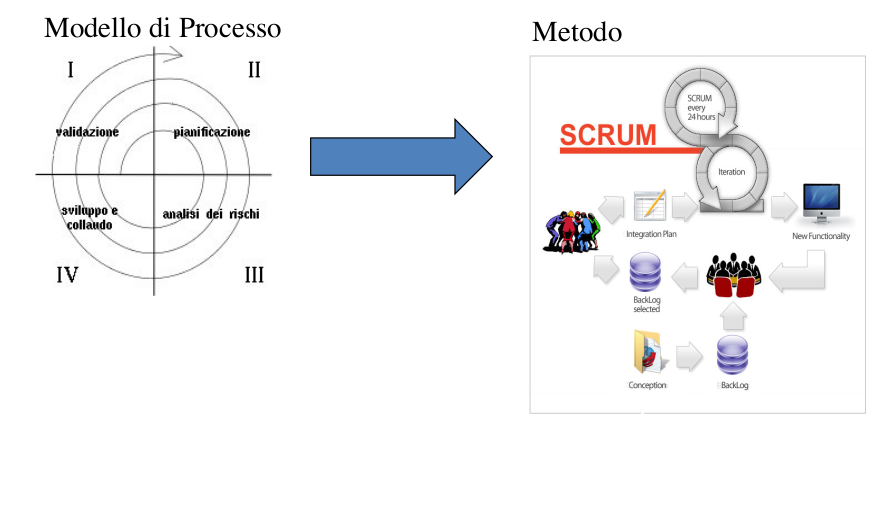
\includegraphics[scale=2.0]{img/ing.png}
\end{center}
Si ha il modello a cascata, inventato da Royce:
\begin{figure}
\label{Modello Cascata}
\psscalebox{1.0 1.0} % Change this value to rescale the drawing.
{
\begin{pspicture}(0,-3.755)(9.11,3.755)
\rput[bl](0.0,3.445){feasibilty study}
\rput[bl](1.2,2.245){requirements analysis \& specification}
\rput[bl](2.8,1.045){design}
\rput[bl](3.6,-0.155){coding \& unit test}
\rput[bl](4.4,-1.355){integration \& system test}
\rput[bl](6.0,-2.555){deployment}
\rput[bl](7.2,-3.755){maintenance}
\psline[linecolor=black, linewidth=0.04, arrowsize=0.05291667cm 2.0,arrowlength=1.4,arrowinset=0.0]{->}(1.2,3.445)(2.0,2.645)
\psline[linecolor=black, linewidth=0.04, arrowsize=0.05291667cm 2.0,arrowlength=1.4,arrowinset=0.0]{->}(2.4,2.245)(3.2,1.445)
\psline[linecolor=black, linewidth=0.04, arrowsize=0.05291667cm 2.0,arrowlength=1.4,arrowinset=0.0]{->}(3.6,1.045)(4.4,0.245)
\psline[linecolor=black, linewidth=0.04, arrowsize=0.05291667cm 2.0,arrowlength=1.4,arrowinset=0.0]{->}(4.8,-0.155)(5.6,-0.955)
\psline[linecolor=black, linewidth=0.04, arrowsize=0.05291667cm 2.0,arrowlength=1.4,arrowinset=0.0]{->}(6.0,-1.355)(6.8,-2.155)
\psline[linecolor=black, linewidth=0.04, arrowsize=0.05291667cm 2.0,arrowlength=1.4,arrowinset=0.0]{->}(7.2,-2.555)(8.0,-3.355)
\end{pspicture}
}
\end{figure}
si ha il seguente feedback del modello a cascata:
\begin{center}
\psscalebox{1.0 1.0} % Change this value to rescale the drawing.
{
\begin{pspicture}(0,-3.8)(15.6,3.8)
\psframe[linecolor=black, linewidth=0.04, dimen=outer](2.8,3.8)(0.0,2.6)
\psframe[linecolor=black, linewidth=0.04, dimen=outer](6.0,2.2)(2.8,1.0)
\psframe[linecolor=black, linewidth=0.04, dimen=outer](9.2,0.6)(6.0,-0.6)
\psframe[linecolor=black, linewidth=0.04, dimen=outer](12.4,-1.0)(9.2,-2.2)
\psframe[linecolor=black, linewidth=0.04, dimen=outer](15.6,-2.6)(12.4,-3.8)
\rput[bl](0.53333336,3.3){definizione}
\rput[bl](0.43333334,2.82){dei requisiti}
\rput[bl](2.8990476,1.76){progettazione}
\rput[bl](3.1866667,1.46){del sistema e}
\rput[bl](6.087619,0.0){implementazione}
\rput[bl](6.0804764,-0.44){e test delle unità}
\rput[bl](9.546667,-1.52){integrazione e }
\rput[bl](9.486667,-2.0){test del sistema}
\rput[bl](13.066667,-3.22){operatività}
\rput[bl](12.646667,-3.5){emanutenzione}
\rput[bl](3.58,1.14){del software}
\psline[linecolor=black, linewidth=0.04, arrowsize=0.05291667cm 2.0,arrowlength=1.4,arrowinset=0.0]{->}(12.4,-3.4)(1.2,-3.4)(1.2,2.6)
\psline[linecolor=black, linewidth=0.04, arrowsize=0.05291667cm 2.0,arrowlength=1.4,arrowinset=0.0]{->}(10.8,-3.4)(10.8,-2.2)
\psline[linecolor=black, linewidth=0.04, arrowsize=0.05291667cm 2.0,arrowlength=1.4,arrowinset=0.0]{->}(7.6,-3.4)(7.6,-0.6)
\psline[linecolor=black, linewidth=0.04, arrowsize=0.05291667cm 2.0,arrowlength=1.4,arrowinset=0.0]{->}(4.4,-3.4)(4.4,1.0)
\psline[linecolor=black, linewidth=0.04, arrowsize=0.05291667cm 2.0,arrowlength=1.4,arrowinset=0.0]{->}(2.8,3.4)(4.4,3.4)(4.4,2.2)
\psline[linecolor=black, linewidth=0.04, arrowsize=0.05291667cm 2.0,arrowlength=1.4,arrowinset=0.0]{->}(6.0,1.8)(7.6,1.8)(7.6,0.6)
\psline[linecolor=black, linewidth=0.04, arrowsize=0.05291667cm 2.0,arrowlength=1.4,arrowinset=0.0]{->}(9.2,0.2)(10.8,0.2)(10.8,-1.0)
\psline[linecolor=black, linewidth=0.04, arrowsize=0.05291667cm 2.0,arrowlength=1.4,arrowinset=0.0]{->}(12.4,-1.4)(14.0,-1.4)(14.0,-2.6)
\end{pspicture}
}
\end{center}
\begin{center}

\psscalebox{1.0 1.0} % Change this value to rescale the drawing.
{
\begin{pspicture}(0,-2.55)(6.71,2.55)
\rput[bl](0.0,2.25){requirements}
\rput[bl](1.6,1.05){design}
\rput[bl](2.4,-0.15){implementation}
\rput[bl](4.0,-1.35){verification}
\rput[bl](4.8,-2.55){maintenance}
\psline[linecolor=black, linewidth=0.04, arrowsize=0.05291667cm 2.0,arrowlength=1.4,arrowinset=0.0]{->}(1.2,2.25)(2.0,1.45)
\psline[linecolor=black, linewidth=0.04, arrowsize=0.05291667cm 2.0,arrowlength=1.4,arrowinset=0.0]{->}(2.4,1.05)(3.2,0.25)
\psline[linecolor=black, linewidth=0.04, arrowsize=0.05291667cm 2.0,arrowlength=1.4,arrowinset=0.0]{->}(3.6,-0.15)(4.4,-0.95)
\psline[linecolor=black, linewidth=0.04, arrowsize=0.05291667cm 2.0,arrowlength=1.4,arrowinset=0.0]{->}(4.8,-1.35)(5.6,-2.15)
\end{pspicture}
}

\end{center}
Invece di rilasciare il sistema in una singola consegna,
sviluppo e consegna sono strutturati in una sequenza di
incrementi, ognuno dei quali corrispondenti a parte
delle funzionalità richieste. Questa è la \textbf{consegna incrementale}. requisiti utente sono ordinati per priorità, i requisiti ad alta priorità sono inclusi nei primi incrementi.  \newpage
Una volta che lo sviluppo di un incremento inizia, i
requisiti sono congelati; invece possono evolvere i
requisiti per gli incrementi successivi:
\begin{center}
\psscalebox{1.0 1.0} % Change this value to rescale the drawing.
{
\begin{pspicture}(0,-2.8)(16.05,2.8)
\rput[bl](0.4,2.4){definizione}
\rput[bl](0.4,2.0){sommaria}
\rput[bl](0.4,1.6){dei requisiti}
\rput[bl](4.4,2.4){assegnazione}
\rput[bl](4.4,2.0){dei requisiti}
\rput[bl](4.4,1.6){agli incrementi}
\rput[bl](8.8,2.4){progettazione}
\rput[bl](8.8,2.0){architettura}
\rput[bl](8.8,1.6){di sistema}
\rput[bl](0.4,-0.4){sviluppo}
\rput[bl](0.4,-0.8){degli incrementi}
\rput[bl](0.4,-1.2){di sistema}
\rput[bl](4.8,-0.4){convalida}
\rput[bl](4.8,-0.8){dell'incremento}
\rput[bl](9.2,-0.4){integrazione}
\rput[bl](9.2,-0.8){dell'incremento}
\rput[bl](13.6,-0.4){validazione}
\rput[bl](13.6,-0.8){del sistema}
\rput[bl](14.0,1.6){sistema finale}
\rput[bl](6.8,-2.8){sistema incompleto}
\psframe[linecolor=black, linewidth=0.04, dimen=outer](2.8,2.8)(0.0,1.2)
\psframe[linecolor=black, linewidth=0.04, dimen=outer](7.2,2.8)(4.0,1.2)
\psframe[linecolor=black, linewidth=0.04, dimen=outer](11.2,2.8)(8.4,1.2)
\psframe[linecolor=black, linewidth=0.04, dimen=outer](3.2,0.0)(0.0,-1.6)
\psframe[linecolor=black, linewidth=0.04, dimen=outer](7.6,0.0)(4.4,-1.6)
\psframe[linecolor=black, linewidth=0.04, dimen=outer](12.0,0.0)(8.8,-1.6)
\psframe[linecolor=black, linewidth=0.04, dimen=outer](16.0,0.0)(13.2,-1.6)
\psline[linecolor=black, linewidth=0.04, arrowsize=0.05291667cm 2.0,arrowlength=1.4,arrowinset=0.0]{->}(2.8,2.0)(4.0,2.0)
\psline[linecolor=black, linewidth=0.04, arrowsize=0.05291667cm 2.0,arrowlength=1.4,arrowinset=0.0]{->}(7.2,2.0)(8.4,2.0)
\psline[linecolor=black, linewidth=0.04, arrowsize=0.05291667cm 2.0,arrowlength=1.4,arrowinset=0.0]{->}(10.0,1.2)(10.0,0.8)(1.2,0.8)(1.2,0.0)
\psline[linecolor=black, linewidth=0.04, arrowsize=0.05291667cm 2.0,arrowlength=1.4,arrowinset=0.0]{->}(3.2,-0.8)(4.4,-0.8)
\psline[linecolor=black, linewidth=0.04, arrowsize=0.05291667cm 2.0,arrowlength=1.4,arrowinset=0.0]{->}(7.6,-0.8)(8.8,-0.8)
\psline[linecolor=black, linewidth=0.04, arrowsize=0.05291667cm 2.0,arrowlength=1.4,arrowinset=0.0]{->}(12.0,-0.8)(13.2,-0.8)
\psline[linecolor=black, linewidth=0.04, arrowsize=0.05291667cm 2.0,arrowlength=1.4,arrowinset=0.0]{->}(14.8,-1.6)(14.8,-2.4)(2.0,-2.4)(2.0,-1.6)
\psline[linecolor=black, linewidth=0.04, arrowsize=0.05291667cm 2.0,arrowlength=1.4,arrowinset=0.0]{->}(14.8,0.0)(14.8,1.6)
\end{pspicture}
}

\end{center}
Con la consegna incrementale si hanno i seguenti vantaggi:
\begin{itemize}
\item funzioni utili per il cliente possono essere rilasciate ad ogni incremento, quindi alcune funzionalità di sistema sono disponibili sin dai primi incrementi
\item i primi incrementi rappresentano dei prototipi che supportano la scoperta dei requisiti per i successivi incrementi
\item i rischi di fallimento si abbassano
\item i servizi a priorità più alta tendono ad essere collaudati più a fondo
\end{itemize}
Se si ha che i requisiti vengono scoperti attraverso lo sviluppo si ha lo \textbf{sviluppo evoluzionistico}. Si usano prototipi che poi non verranno utilizzati nel corso del progetto vero e proprio\\
\begin{center}
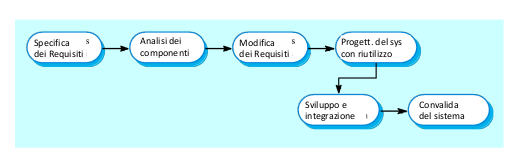
\includegraphics[scale=0.7]{img/ms.png}
\end{center}
Si ha ingegneria del software basata su componenti se si hanno già librerie su cui lavorare.\\
Passiamo al primo modello iterativo, quello di B. Boehm.
\begin{center}
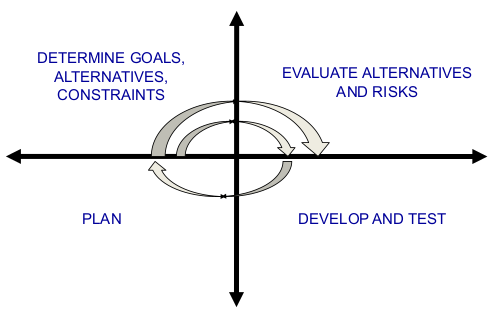
\includegraphics[scale=0.7]{img/ms2.png}
\end{center}
si parte dal quadrante in alto a sinistra e si arriva al prodotto finale mediante una serie di iterazioni. Si sceglie ovviamente la soluzione più sicura. I vari passaggi sono qui rappresentati:
\begin{center}
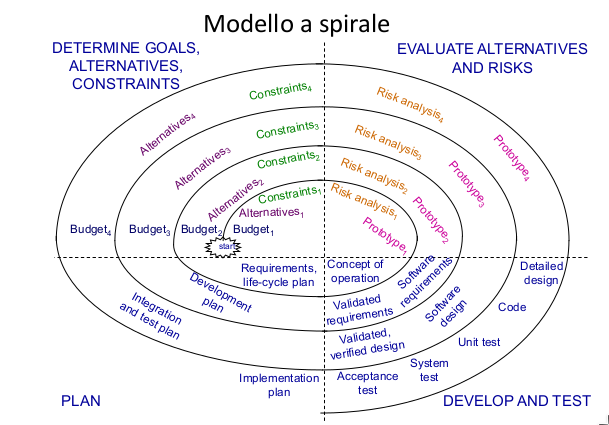
\includegraphics[scale=0.7]{img/ms3.png}
\end{center}
\section{Modello UP}
Il metodo di modellazione UP(Unified Process), conosciuto anche come RUP(Rational Unified Process), è un
processo iterativo molto diffuso per lo sviluppo software, in cui sono presenti degli elementi tratti da 
altri metodi, come Extreme Programming, Scrum e così via.

Lo sviluppo iterativo
Si hanno i modelli agili, che si basano sulla \textbf{consegna incrementale}. Si hanno iterazioni brevi e timeboxed, con un raffinamento evolutivo di piani, dei requisiti e del progetto. Questi metodi favoriscono la collaborazione nei gruppi e la riduzione dei costi.
\subsection{Modello UP o RUP}
Il metodo UP, \textit{inified process}, conosciuto anche come RUP, \textit{Rational Unified Process}, usa la notazione UML, \textit{unified modeling language} ed è uno dei più importanti modelli agili. È è un processo iterativo e incrementale. Si basa sulla suddivisone di un grande processo in iterazioni controllate. Si hanno passi piccoli, timeboxed da 2 a 6 settimane, feedback rapito e adattamento, di requisiti, modelli, stime di sviluppo e costi e priorità.
\begin{center}
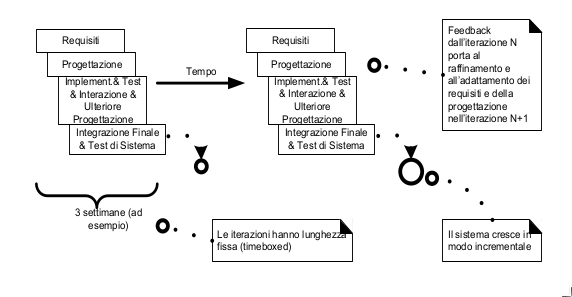
\includegraphics[scale=0.7]{img/ms4.png}
\end{center}
Si hanno 4 fasi nel modello RUP:
\begin{enumerate}
\item \textbf{avviamento:} dove viene stabilita la “bussines rationale” del progetto e stabiliti gli obiettivi, stime dei costi e dei tempi. Si ha uno studio di fattibilità, \textit{Life-Cycle Objective Milestone}
\item \textbf{elaborazione}: dove si raccolgono i requisiti in modo più dettagliato, si procede con l'analisi ad alto livello per stabilire l'architettura di base e vengono analizzati i rischi principali. Si hanno stime più affidabili: \textit{Life-Cycle Architecture Milestone}
\item \textbf{costruzione} che consiste di molte iterazioni, e ad ogni iterazione viene costruita una parte del sistema che soddisfa un sottoinsieme di requisiti. Viene effettuato il testing e l'integrazione. Si ha la preparazione al rilascio: \textit{Initial Operational Capability Milestone}
\item \textbf{transizione:} dove vengono affrontati tutti gli aspetti legati al fine-tuning delle funzionalità,
prestazioni, qualità, beta-testing, ottimizzazione, formazione degli
utenti,... È la \textit{Product Release Milestone}
\end{enumerate}
\begin{center}
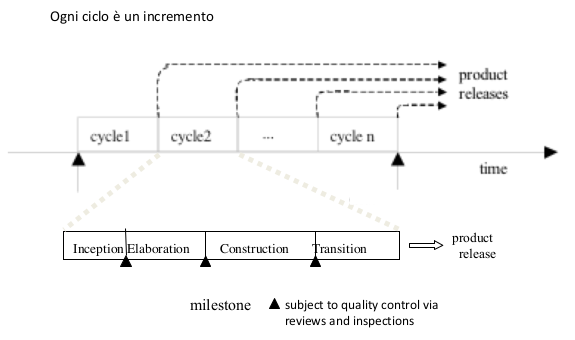
\includegraphics[scale=0.7]{img/ms5.png}
\end{center}
Si hanno i seguenti vantaggi dello sviluppo iterativo:
\begin{itemize}
\item minore chance di fallimento del progetto
\item riduzione precoce dei rischi
\item progresso visibile
\item feedback precoce e coinvolgimento dell'utente
\item "abbracciare il cambiamento"
\end{itemize}
\begin{center}
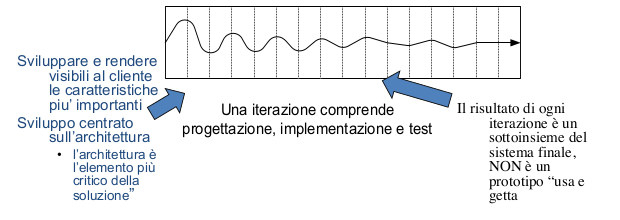
\includegraphics[scale=0.7]{img/ms6.png}
\end{center}
Vediamo un esempio con 5 iterazioni:
\begin{center}
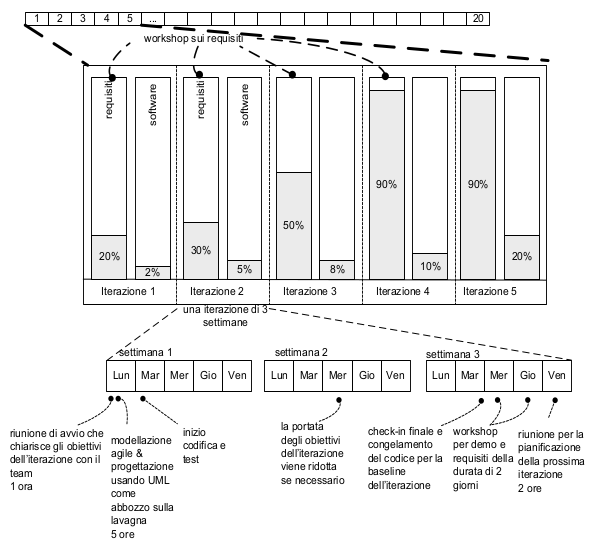
\includegraphics[scale=0.7]{img/ms7.png}
\end{center}
\newpage
vediamo un'altra rappresentazione del ciclo di sviluppo:
\begin{center}
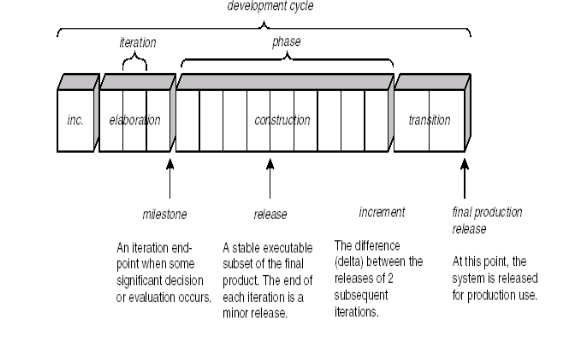
\includegraphics[scale=0.65]{img/ms8.png}
\end{center}
vediamo anche un'immagine per rappresentare l'organizzazione del processo, con fasi, iterazioni e "discipline":
\begin{center}
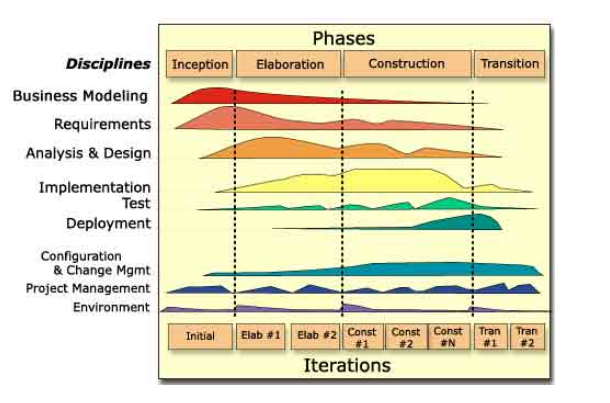
\includegraphics[scale=0.65]{img/ms9.png}
\end{center}
tra le discipline troviamo analisi e progettazione
%approfondire su libro
Si hanno le seguenti caratteristiche principlai per l?UP:
\begin{itemize}
\item è iterativo e incrementale
\item si enfasi sul modello invece che sul linguaggio naturale
\item è centrato sull'architettura
\end{itemize}
\subsection{Processo Scrum}
Iniziamo con un'immagine che rappresenta questo metodo agile:
\begin{center}
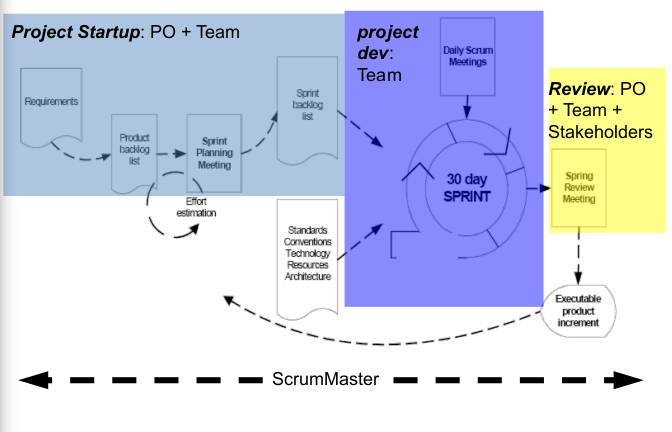
\includegraphics[scale=0.65]{img/ms10.png}
\end{center}
È un processo iterativo basato sull controllo dello stato di
avanzamento. Si hanno i seguenti principi fondamentali:
\begin{itemize}
\item \textbf{visibilità:} gli aspetti significativi del processo di sviluppo devono essere visibili a tutti e tutti gli aspetti devono essere chiari
\item \textbf{ispezione:} poter ispezionare frequentemente il lavoro fatto per verificare che si sta procedendo verso gli
obiettivi posti
\item \textbf{adattamento}, se si sta deviando dagli obiettivi, occorre un adattamento per minimizzare altre deviazioni. Deve essere svolto nel minor tempo possibile in caso di necessità
\end{itemize}
Si hanno i seguenti ruoli:
\begin{itemize}
\item \textbf{product owner} che si occupa della definizione delle
caratteristiche del progetto da sviluppare (1 sola
persona, e.g. committente, o altri...); gestisce il
Product Backlog. Lavora costantemente col team
\item \textbf{team:} dedicato allo sviluppo e rilascio del
prodotto attraverso incrementi successivi (da 3 a
7/8 membri)
\item \textbf{scrum master:} responsabile che lo SCRUM venga
applicato correttamente. Non è un project manager, fa da intermezzo tra team e product owner, collabora col team etc
\end{itemize}
Ecco un'immagine che rappresenta lo sviluppo con Scrum:
\begin{center}
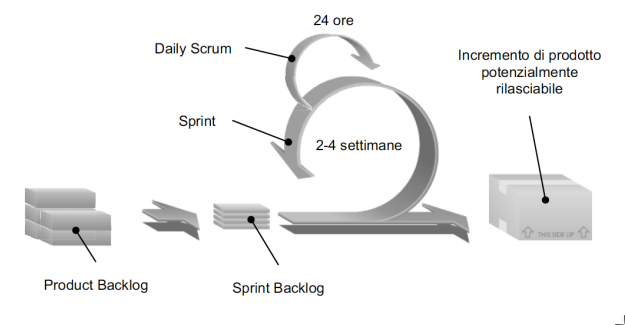
\includegraphics[scale=0.7]{img/ms11.png}
\end{center}
SI hanno quindi:
\begin{itemize}
\item releases brevi con sottoinsiemi consegnati velocemente
\item in ogni istante si hanno test eseguibili, non si ha logica duplicata e si ha un numero minimo di features
\item si ha \textit{refactoring }con miglioramento continuo
\item si un testo continuo e automatico, \textit{testing first}
\item si hanno due sviluppatori che lavorano insieme, \textit{pair programming}
\item il codice è proprietà del team e non del singolo dev, \textit{collective owbership}
\item si hanno check-in frequenti e integrazioni continue, \textit{continuous integration}
\item il cliente lavora col team
\end{itemize}
I \textbf{requisiti} sono una descrizione dei servizi del sistema e dei suoi vincoli operativi. Si hanno due tipi di requisiti:
\begin{itemize}
\item \textbf{requisiti utenti:} affermazioni in linguaggio naturale, corredate da tabelle e diagrammi, riguardanti i servizi che il sistema offre ed i vincoli operazionali. Sono scritti per i clienti e sono da loro comprensibili anche se non	hanno conoscenze tecniche dettagliate.\\

\item \textbf{requisiti di sistema:} un documento strutturato che definisce in modo dettagliato le funzioni del sistema, i servizi ed i vincoli operazionali. Definisce cosa deve essere implementato, quindi può essere parte del
contratto tra acquirente e sviluppatore. È la base del progetto della soluzione e può essere illustrato utilizzando i \textbf{modelli di sistema}.

\end{itemize}
i requisiti possono avere 3 problemi:
\begin{itemize}
\item \textbf{ambiguità:} il sistema fornisce visualizzazioni appropriate per leggere i documenti
\item \textbf{incompletezza:} i requisiti devono descrivere tutti i	servizi forniti dal sistema (anche se in realtà tutto ciò è impossibile, per questo esistono i cambiamenti)
\item \textbf{inconsistenza}: le descrizioni non devono contenere conflitti o contraddizioni (anche questa cosa è difficilissima da ottenere)
\end{itemize}
SI hanno anche i \textbf{requisiti funzionali} servizi che il sistema deve (o non deve) fornire. Si hanno anche i \textit{requisiti non funzionali}, come vincoli sui servizi temporali, standard, sull'usabilità etc... I requisiti non funzionali possono essere più critici dei requisiti funzionali: \textbf{se non sono soddisfatti il sistema è spesso inutilizzabile}. Si hanno alcuni requisiti non funzionali:
\begin{itemize}
\item \textbf{prodotto: }specificano che il prodotto deve comportarsi in un modo particolare
esempi: velocità di esecuzione, affidabilità.\\
\textit{L’interfaccia utente sarà implementata con HTML semplice senza frames
e applets}
\item \textbf{organizzativi: }conseguenza di politiche e procedure dell’organizzazione del cliente e dello sviluppatore.
esempi: linguaggio di programmazione, metodo di sviluppo.\\
\textit{Il processo di sviluppo e la relativa documentazione sarà conforme alle
norme XYZCo-SP-STAN-95}
\item \textbf{esterni: }provengono da fattori esterni al sistema e al processo di sviluppo.
esempi: interoperabilità, leggi e norme.
\\ \textit{Il sistema non deve rilevare agli operatori nessuna informazione
personale sui clienti oltre al nome e al numero di riferimento}
\end{itemize}
\begin{center}
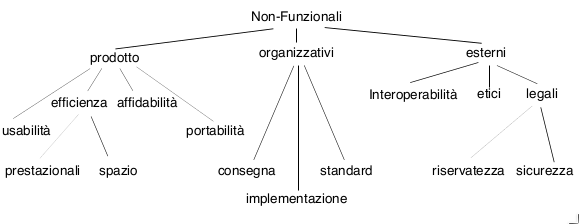
\includegraphics[scale=0.8]{img/req.png}
\end{center}
\newpage
Tutto ciò perché il linguaggio naturale presenta mancanza di chiarezza, ambiguità, confusione etc... Esistono alternative:
\begin{center}
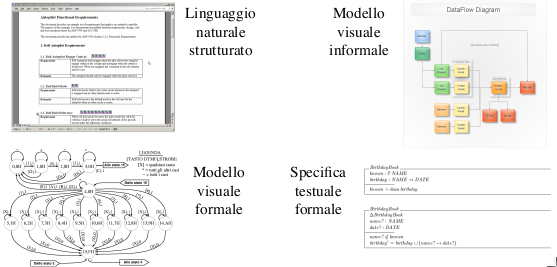
\includegraphics[scale=0.8]{img/req2.png}
\end{center}
I requisiti hanno un formato standard, usano il linguaggio in modo consistente, evitano il gergo tecnico e evidenziano delle porzioni di testo per identificare le parti più importanti dei requisiti. Un esempio di standard è quello IEEE830.\\
I casi d'uso possono essere visualizzati con l'UML:
\begin{center}
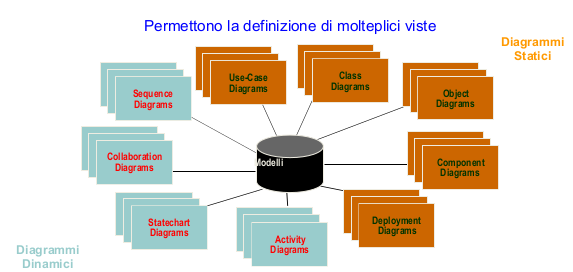
\includegraphics[scale=0.8]{img/uml.png}
\end{center}

\chapter{Analisi dei Requisiti e Casi d'uso}
Si hanno i cosiddetti \textbf{casi d'uso}, che ci indicano una possibile situazione, infatti \textit{documentano requisiti funzionali
complementari alla lista dei requisiti non-funzionali
punto di partenza per analisi e progettazione}. SI hanno i seguenti elementi fondamentali dei casi d'uso:
\begin{itemize}
\item \textbf{attori}, divisi in:
\begin{itemize}
\item \textbf{attore primario:} raggiunge degli obiettivi utente utilizzando i servizi del sistema
\item \textbf{attore di supporto:} offre un servizio, spesso è un sistema informatico, ma può essere anche una organizzazione o una persona
\item \textbf{attore fuori scena:} ha un interesse nel caso d'uso, ma non è né un attore primario né di supporto
\end{itemize}
\item \textbf{scenari}
\end{itemize}
qualora manchino scenari alternativi si ha il cosiddetto \textbf{formato informale}.\\
Nello studio dei casi d'uso bisogna concentrasi sullo scopo dell'autore e su cosa deve fare effettivamente il sistema (\textit{responsabilità}). Bisogna ignorare invece l'interfaccia utente e come effettivamente lo fa il sistema. \\
Si hanno i cosiddetti 3 test:
\begin{itemize}
\item \textbf{test del capo:} \textit{Il capo chiede: "Cosa avete fatto tutto il giorno?"
Voi rispondere con il nome del caso d'uso. Sarà
soddisfatto?}
\item \textbf{test EBP (\textit{Elementary Business Process}:} \textit{attività che aggiunge un valore di business misurabile e lascia i dati in uno stato coerente}
\item \textbf{test della dimensione:} > 1 azione
(da 3 a 10 pagine nel formato dettagliato)
\end{itemize}
Attività secondari e piccoli passi possono
diventare casi d'uso per evitare le ripetizioni del
testo, in questo caso i tre test possono essere
violati. I diagrammi, con il nome del caso d'uso, le relazioni e gli attori, sono secondari, \textbf{i casi d'uso sono documenti di testo}. Vediamo un esempio:
\begin{center}
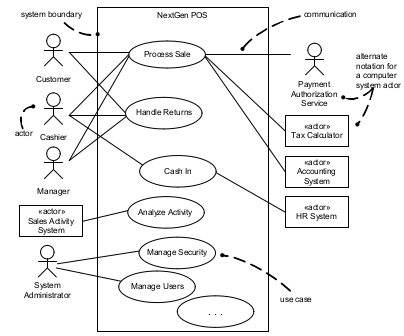
\includegraphics[scale=0.8]{img/cas.png}
\end{center}
Le \textbf{associazioni} sono un canale di comunicazione tra attore e caso d'uso. Sono rappresentate:
\begin{itemize}
\item \textbf{una linea direzionata} per specificare chi da inizio all'iterazione
\item \textbf{una linea semplice} per indicare che entrambe le parti possono dare inizio all'iterazione
\end{itemize} 
\begin{center}
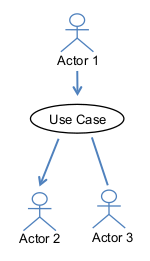
\includegraphics[scale=0.7]{img/ass.png}
\end{center}
\begin{center}
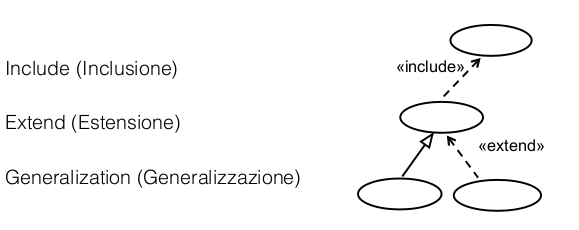
\includegraphics[scale=0.7]{img/ass3.png}
\end{center}
L'\textbf{include} è una relazione tra un caso d'uso base ed un caso d'uso incluso nel caso d'uso base il cui comportamento definito nel caso d'uso
\textit{inclusion} esplicitamente incluso nel caso
d'uso base. Per l'\textit{include} si ha che il caso d'uso è eseguito completamente quando viene
raggiunto il punto di inclusione.\\
L'\textbf{extend} connette un caso d'uso esteso ad un
caso d'uso base. Aggiunge varianti ad un caso d'uso
base. Viene inserito solo se la condizione di
estensione è vera. Estensione inserite solo in
corrispondenza degli \textit{extension point}.
\begin{center}
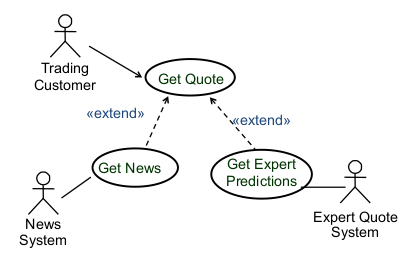
\includegraphics[scale=0.7]{img/ex.png}
\end{center}
\begin{center}
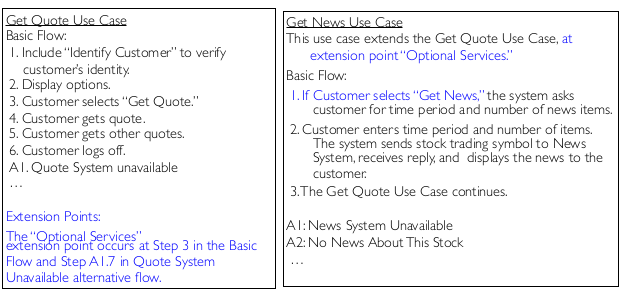
\includegraphics[scale=0.7]{img/ex2.png}
\end{center}
Per l'\textit{include} si ha che caso d'uso esteso è eseguito quando il punto di estensione è
raggiunto e la condizione di estensione è vera.\\
Un caso d'uso base è una \textbf{generalizzazione} di
un caso d'uso child. Viene eseguito se la condizione di
generalizzazione è vera. La generalizzazione è puramente concettuale, non ci sono regole da seguire, come ad
esempio l'utilizzo di punti di estensione:
\begin{center}
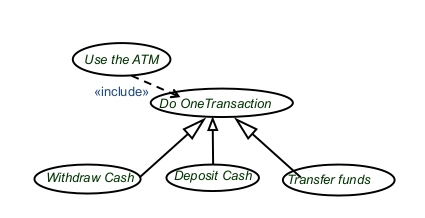
\includegraphics[scale=0.7]{img/gen.png}
\end{center}
La \textit{generalizzazione} collega un attore child ad un attore parent. Gli attori child partecipano a tutti i casi d'uso in cui partecipano il parent:
\begin{center}
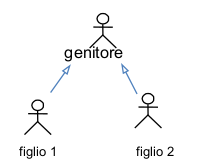
\includegraphics[scale=0.7]{img/gen2.png}
\end{center}
\begin{center}
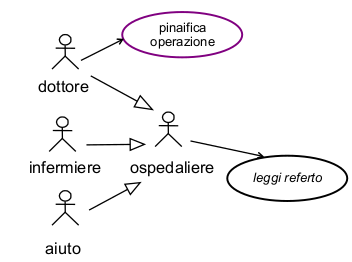
\includegraphics[scale=0.7]{img/gen3.png}
\end{center}
\end{document}
